\subsection{Laurent展開}

	いま$R$を正の実数とし,$f$を
	\begin{align}
		\Omega \defeq \disc{0}{R} \backslash \{0\}
	\end{align}
	上の正則関数とする.また$z$を$\Omega$の要素とし,$r$と$\rho$を
	\begin{align}
		r < |z| < \rho < R
	\end{align}
	を満たす正の実数とする.このとき
	\begin{align}
		[0,1] \ni t \longmapsto \rho \cdot e^{2 \cdot \pi \cdot \isym \cdot t}
	\end{align}
	なる路を$\gamma$とし,
	\begin{align}
		[0,1] \ni t \longmapsto r \cdot e^{2 \cdot \pi \cdot \isym \cdot t}
	\end{align}
	なる路を$\eta$とすれば,
	\begin{align}
		f(z) = \frac{1}{2 \cdot \pi \cdot \isym} \cdot 
		\left[-\int_{\eta} \frac{f(\zeta)}{\zeta-z}\ d\zeta + \int_{\gamma} \frac{f(\zeta)}{\zeta-z}\ d\zeta\right]
		\label{fom:Laurent_series_1}
	\end{align}
	が成立する.
	
	細かいところは後に回して概略を説明する.いま
	\begin{align}
		\alpha \defeq \pvarg{z} + \pi
	\end{align}
	及び
	\begin{align}
		\beta \defeq \frac{\alpha}{2 \cdot \pi}
	\end{align}
	とおき,$\theta$を$\eta$の逆路とし,$[0,4]$上の路$\xi$を
	\begin{align}
		t \longmapsto
		\begin{cases}
			\gamma(t) & \mbox{if } 0 \leq t \leq \beta \\
			\seg{\rho \cdot e^{\isym \cdot \alpha}}{r \cdot e^{\isym \cdot \alpha}}(t-\beta) & \mbox{if } \beta \leq t \leq \beta + 1 \\
			\theta(t-\beta-1) & \mbox{if } \beta + 1 \leq t \leq \beta + 2 \\
			 \seg{r \cdot e^{\isym \cdot \alpha}}{\rho \cdot e^{\isym \cdot \alpha}}(t-\beta-2) & \mbox{if } \beta + 2 \leq t \leq \beta + 3 \\
			\gamma(t-\beta-3) & \mbox{if } \beta + 3 \leq t \leq 4
		\end{cases}
	\end{align}
	なる関係により定める.イメージとしては,$\xi$は始め
	
	\begin{center}
		\begin{tikzpicture}
			\node [anchor=north] at (0,0) {$0$};
			\node [anchor=west] at ({sqrt(2)},{sqrt(2)}) {$z$};
			\draw [domain=0:2*pi, samples=200, dotted] plot({3*cos(\x r)},{3*sin(\x r)});
			\foreach \Point in {({sqrt(2)},{sqrt(2)})}{
				\node at \Point {\textbullet};
			}
			\draw [domain=0:(5*pi/4), thick, samples=200, color=red] plot({2.5*cos(\x r)},{2.5*sin(\x r)});
			\draw [thick, color=red, ->] ({-2.5/sqrt(2)},{-2.5/sqrt(2)}) -- ({-1/sqrt(2)},{-1/sqrt(2)});
			
			\draw [domain=0:(5*pi/4), samples=200, ->] plot({0.5*cos(\x r)},{0.5*sin(\x r)});
			\draw [dotted] (0,0) -- (2.5,0);
			\draw [dotted] ({sqrt(2)},{sqrt(2)}) -- ({-2.5/sqrt(2)},{-2.5/sqrt(2)});
			\node [anchor=north west] at ({cos(3*pi/4 r)},{sin(3*pi/4 r)}) {$\alpha$};
		\end{tikzpicture}
	\end{center}
	
	を描き,次は
	
	\begin{center}
		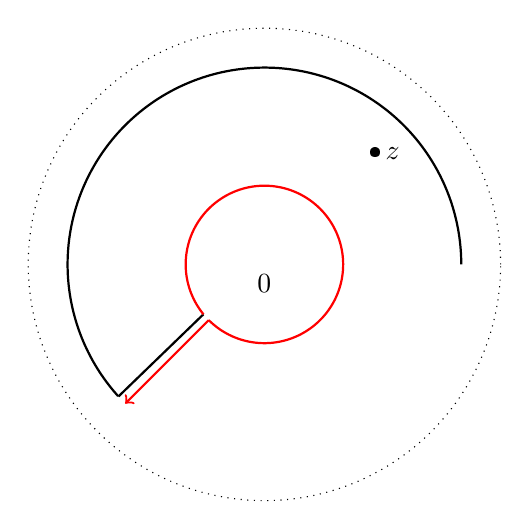
\begin{tikzpicture}
			\node [anchor=north] at (0,0) {$0$};
			\node [anchor=west] at ({sqrt(2)},{sqrt(2)}) {$z$};
			\draw [domain=0:2*pi, samples=200, dotted] plot({3*cos(\x r)},{3*sin(\x r)});
			\foreach \Point in {({sqrt(2)},{sqrt(2)})}{
				\node at \Point {\textbullet};
			}
			\draw [domain=0:(5*pi/4)-0.05, thick, samples=200] plot({2.5*cos(\x r)},{2.5*sin(\x r)});
			\draw [thick] ({2.5*cos((5*pi/4-0.05) r)},{2.5*sin((5*pi/4-0.05) r)}) -- ({cos((5*pi/4-0.1) r)},{sin((5*pi/4-0.1) r)});
			\draw [domain=5*pi/4-0.1:-3*pi/4, thick, color=red, samples=200] plot({cos(\x r)},{sin(\x r)});
			\draw [thick, color=red, ->] ({-1/sqrt(2)},{-1/sqrt(2)}) -- ({-2.5/sqrt(2)},{-2.5/sqrt(2)});
		\end{tikzpicture}
	\end{center}
	
	を描き,最後に
	
	\begin{center}
		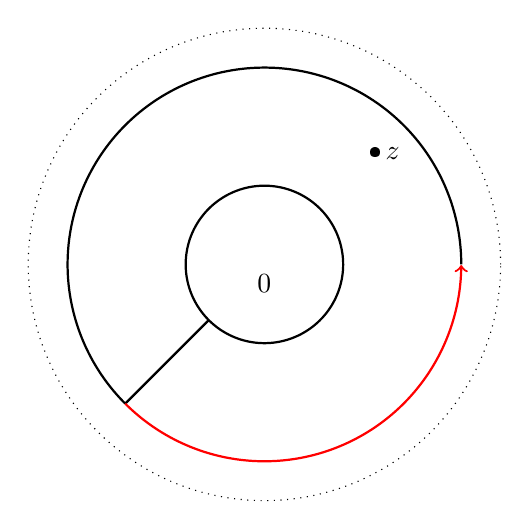
\begin{tikzpicture}
			\node [anchor=north] at (0,0) {$0$};
			\node [anchor=west] at ({sqrt(2)},{sqrt(2)}) {$z$};
			\draw [domain=0:2*pi, samples=200, dotted] plot({3*cos(\x r)},{3*sin(\x r)});
			\foreach \Point in {({sqrt(2)},{sqrt(2)})}{
				\node at \Point {\textbullet};
			}
			\draw [domain=0:(5*pi/4), thick, samples=200] plot({2.5*cos(\x r)},{2.5*sin(\x r)});
			\draw [thick] ({-2.5/sqrt(2)},{-2.5/sqrt(2)}) -- ({-1/sqrt(2)},{-1/sqrt(2)});
			\draw [domain=(-3*pi/4):(5*pi/4), thick, samples=200] plot({cos(5*pi/4-\x r)},{sin(5*pi/4-\x r)});
			\draw [thick] ({-1/sqrt(2)},{-1/sqrt(2)}) -- ({-2.5/sqrt(2)},{-2.5/sqrt(2)});
			\draw [domain=(5*pi/4):2*pi, thick, color=red, samples=200, ->] plot({2.5*cos(\x r)},{2.5*sin(\x r)});
		\end{tikzpicture}
	\end{center}
	
	を描く.$\xi$の回転数は,$\C \backslash \disc{0}{R}$の要素$w$に対しては
	\begin{align}
		\Wnd_{\xi}(w) = 0,
		\label{fom:Laurent_series_2}
	\end{align}
	また原点においても
	\begin{align}
		\Wnd_{\xi}(0) = 0,
		\label{fom:Laurent_series_3}
	\end{align}
	他方で$z$に対しては
	\begin{align}
		\Wnd_{\xi}(z) = 1
		\label{fom:Laurent_series_4}
	\end{align}
	が成立する.従ってCauchyの積分定理より
	\begin{align}
		f(z) = \frac{1}{2 \cdot \pi \cdot i} \cdot \int_{\xi} \frac{f(\zeta)}{\zeta - z}\ d\zeta
	\end{align}
	が得られる.ところで
	\begin{align}
		\int_{[0,\beta]} \frac{f \circ \xi}{\xi - z}\ d\mu_{\xi} 
		= \int_{[0,\beta]} \frac{f \circ \gamma}{\gamma - z}\ d\mu_{\gamma}
		\label{fom:Laurent_series_5}
	\end{align}
	かつ
	\begin{align}
		\int_{[\beta,\beta+1]} \frac{f \circ \xi}{\xi - z}\ d\mu_{\xi}
		= \int_{\seg{\rho \cdot e^{\isym \cdot \alpha}}{r \cdot e^{\isym \cdot \alpha}}} \frac{f(\zeta)}{\zeta - z}\ d\zeta
		\label{fom:Laurent_series_6}
	\end{align}
	かつ
	\begin{align}
		\int_{[\beta+1,\beta+2]} \frac{f \circ \xi}{\xi - z}\ d\mu_{\xi}
		= \int_{[0,1]} \frac{f \circ \theta}{\theta - z}\ d\mu_{\theta}
		\label{fom:Laurent_series_7}
	\end{align}
	かつ
	\begin{align}
		\int_{[\beta+2,\beta+3]} \frac{f \circ \xi}{\xi - z}\ d\mu_{\xi}
		= \int_{\seg{r \cdot e^{\isym \cdot \alpha}}{\rho \cdot e^{\isym \cdot \alpha}}} \frac{f(\zeta)}{\zeta - z}\ d\zeta
		\label{fom:Laurent_series_8}
	\end{align}
	かつ
	\begin{align}
		\int_{[\beta+3,4]} \frac{f \circ \xi}{\xi - z}\ d\mu_{\xi}
		= \int_{[\beta,1]} \frac{f \circ \gamma}{\gamma - z}\ d\mu_{\gamma}
		\label{fom:Laurent_series_9}
	\end{align}
	が成り立つので
	\begin{align}
		\int_{\xi} \frac{f(\zeta)}{\zeta - z}\ d\zeta
		&= \int_{[0,\beta]} \frac{f \circ \xi}{\xi - z}\ d\mu_{\xi} 
			+ \int_{[\beta,\beta+1]} \frac{f \circ \xi}{\xi - z}\ d\mu_{\xi}
			+ \int_{[\beta+1,\beta+2]} \frac{f \circ \xi}{\xi - z}\ d\mu_{\xi} \\
			&\quad + \int_{[\beta+2,\beta+3]} \frac{f \circ \xi}{\xi - z}\ d\mu_{\xi}
			+ \int_{[\beta+3,4]} \frac{f \circ \xi}{\xi - z}\ d\mu_{\xi} \\
		&= \int_{[0,\beta]} \frac{f \circ \gamma}{\gamma - z}\ d\mu_{\gamma} 
			+ \int_{\seg{\rho \cdot e^{\isym \cdot \alpha}}{r \cdot e^{\isym \cdot \alpha}}} \frac{f(\zeta)}{\zeta - z}\ d\zeta
			+ \int_{[0,1]} \frac{f \circ \theta}{\theta - z}\ d\mu_{\theta} \\
			&\quad + \int_{\seg{r \cdot e^{\isym \cdot \alpha}}{\rho \cdot e^{\isym \cdot \alpha}}} \frac{f(\zeta)}{\zeta - z}\ d\zeta
			+ \int_{[\beta,1]} \frac{f \circ \gamma}{\gamma - z}\ d\mu_{\gamma} \\
		&= \int_{[0,1]} \frac{f \circ \gamma}{\gamma - z}\ d\mu_{\gamma} + \int_{[0,1]} \frac{f \circ \theta}{\theta - z}\ d\mu_{\theta} \\
		&= \int_{[0,1]} \frac{f \circ \gamma}{\gamma - z}\ d\mu_{\gamma} - \int_{[0,1]} \frac{f \circ \eta}{\eta - z}\ d\mu_{\eta}
	\end{align}
	が成立する.以上で(\refeq{fom:Laurent_series_1})を得る.
	
	\begin{description}
		\item[(\refeq{fom:Laurent_series_2})の略証]
		\item[(\refeq{fom:Laurent_series_3})の略証]
		\item[(\refeq{fom:Laurent_series_4})の略証]
		\item[(\refeq{fom:Laurent_series_5})の略証]
			$\borel{[0,\beta]}$の任意の要素$E$に対して
			\begin{align}
				\mu_{\xi}(E) = \mu_{\gamma}(E)
			\end{align}
			が成り立てば良い.実際,$s$と$t$を
			\begin{align}
				s < t
			\end{align}
			なる$[0,\beta]$の要素とすれば
			\begin{align}
				\mu_{\xi}(]s,t]) = \xi(t) - \xi(s) = \gamma(t) - \gamma(s) = \mu_{\gamma}(]s,t])
			\end{align}
			が成立するので,測度の一致の定理より
			\begin{align}
				\mu_{\xi}\rest_{\borel{[0,\beta]}} = \mu_{\gamma}\rest_{\borel{[0,\beta]}}
			\end{align}
			が従う.
			
		\item[(\refeq{fom:Laurent_series_6})の略証]
			$\varphi$を
			\begin{align}
				[0,1] \ni s \longmapsto s + \beta
			\end{align}
			なる写像とし
			\begin{align}
				\sigma \defeq \xi \rest_{[\beta,\beta+1]}
			\end{align}
			とおけば
			\begin{align}
				\int_{[\beta,\beta+1]} \frac{f \circ \xi}{\xi - z}\ d\mu_{\xi}
				= \int_{[\beta,\beta+1]} \frac{f \circ \sigma}{\sigma - z}\ d\mu_{\sigma}
				= \int_{[0,1]} \frac{f \circ (\sigma \circ \varphi)}{\sigma \circ \varphi - z}\ d\mu_{\sigma \circ \varphi}
			\end{align}
			が成り立つ(P. \pageref{fom:change_of_parameter_interval_complex_contour_integral}).ここで
			\begin{align}
				\sigma \circ \varphi = \seg{\rho \cdot e^{\isym \cdot \alpha}}{r \cdot e^{\isym \cdot \alpha}}
			\end{align}
			であるから
			\begin{align}
				\int_{[0,1]} \frac{f \circ (\sigma \circ \varphi)}{\sigma \circ \varphi - z}\ d\mu_{\sigma \circ \varphi}
				= \int_{\seg{\rho \cdot e^{\isym \cdot \alpha}}{r \cdot e^{\isym \cdot \alpha}}} \frac{f(\zeta)}{\zeta - z}\ d\zeta
			\end{align}
			も成立する.
			
		\item[(\refeq{fom:Laurent_series_7})の略証]
			$\varphi$を
			\begin{align}
				[0,1] \ni s \longmapsto s + \beta + 1
			\end{align}
			なる写像とし
			\begin{align}
				\sigma \defeq \xi \rest_{[\beta+1,\beta+2]}
			\end{align}
			とおけば
			\begin{align}
				\int_{[\beta+1,\beta+2]} \frac{f \circ \xi}{\xi - z}\ d\mu_{\xi}
				= \int_{[\beta+1,\beta+2]} \frac{f \circ \sigma}{\sigma - z}\ d\mu_{\sigma}
				= \int_{[0,1]} \frac{f \circ (\sigma \circ \varphi)}{\sigma \circ \varphi - z}\ d\mu_{\sigma \circ \varphi}
			\end{align}
			が成り立つ(P. \pageref{fom:change_of_parameter_interval_complex_contour_integral}).ここで
			\begin{align}
				\sigma \circ \varphi = \theta
			\end{align}
			であるから
			\begin{align}
				\int_{[0,1]} \frac{f \circ (\sigma \circ \varphi)}{\sigma \circ \varphi - z}\ d\mu_{\sigma \circ \varphi}
				= \int_{[0,1]} \frac{f \circ \theta}{\theta - z}\ d\mu_{\theta}
			\end{align}
			も成立する.
			
		\item[(\refeq{fom:Laurent_series_8})の略証]
			これも(\refeq{fom:Laurent_series_6})や(\refeq{fom:Laurent_series_7})と同様にして得られる.また
			$\seg{r \cdot e^{\isym \cdot \alpha}}{\rho \cdot e^{\isym \cdot \alpha}}$
			は$\seg{\rho \cdot e^{\isym \cdot \alpha}}{r \cdot e^{\isym \cdot \alpha}}$の逆路なので
			\begin{align}
				\int_{\seg{\rho \cdot e^{\isym \cdot \alpha}}{r \cdot e^{\isym \cdot \alpha}}} \frac{f(\zeta)}{\zeta - z}\ d\zeta
				+ \int_{\seg{r \cdot e^{\isym \cdot \alpha}}{\rho \cdot e^{\isym \cdot \alpha}}} \frac{f(\zeta)}{\zeta - z}\ d\zeta 
				= 0
			\end{align}
			が成立する.
			
		\item[(\refeq{fom:Laurent_series_9})の略証]
			$\varphi$を
			\begin{align}
				[\beta,1] \ni s \longmapsto s + 3
			\end{align}
			なる写像とすれば
			\begin{align}
				\int_{[\beta+3,4]} \frac{f \circ \xi}{\xi - z}\ d\mu_{\xi}
				= \int_{[\beta,1]} \frac{f \circ (\xi \circ \varphi)}{\xi \circ \varphi - z}\ d\mu_{\xi \circ \varphi}
			\end{align}
			が成り立つが,他方で
			\begin{align}
				\xi \circ \varphi = \gamma \rest_{[\beta,1]}
			\end{align}
			かつ
			\begin{align}
				\mu_{\gamma} \rest_{\borel{[\beta,1]}} = \mu_{\gamma \rest_{[\beta,1]}}
			\end{align}
			が成り立つので
			\begin{align}
				\int_{[\beta,1]} \frac{f \circ (\xi \circ \varphi)}{\xi \circ \varphi - z}\ d\mu_{\xi \circ \varphi}
				= \int_{[\beta,1]} \frac{f \circ \gamma \rest_{[\beta,1]}}{\gamma \rest_{[\beta,1]} - z}\ d\mu_{\gamma \rest_{[\beta,1]}}
				= \int_{[\beta,1]} \frac{f \circ \gamma}{\gamma - z}\ d\mu_{\gamma}
			\end{align}
			が従う.
	\end{description}